\documentclass{article}

\usepackage{times}
\usepackage{graphicx} % more modern
\usepackage{subfigure} 
\usepackage{natbib}
\usepackage{algorithm}
\usepackage{algorithmic}
\usepackage{hyperref}
\newcommand{\theHalgorithm}{\arabic{algorithm}}

% Employ the following version of the ``usepackage'' statement for
% submitting the draft version of the paper for review.  This will set
% the note in the first column to ``Under review.  Do not distribute.''
%\usepackage{icml2015stylefiles/icml2015} 

% Employ this version of the ``usepackage'' statement after the paper has
% been accepted, when creating the final version.  This will set the
% note in the first column to ``Proceedings of the...''
\usepackage[accepted]{icml2015stylefiles/icml2015}


% The \icmltitle you define below is probably too long as a header.
% Therefore, a short form for the running title is supplied here:
\icmltitlerunning{Submission and Formatting Instructions for ICML 2015}

\begin{document} 

\twocolumn[
\icmltitle{Sparse Neural Networks:\\
 Improving Feedforward Neural Network Efficiency with Sparse Matrix Constructions}

% It is OKAY to include author information, even for blind
% submissions: the style file will automatically remove it for you
% unless you've provided the [accepted] option to the icml2015
% package.
\icmlauthor{Dr, Choromanski}{email@yourdomain.edu}
\icmladdress{Google Research, NY}
\icmlauthor{Alfred Bou\'{e}rly}{email@coauthordomain.edu}
\icmladdress{Columbia University}
\icmlauthor{Patrick Boueri}{email@coauthordomain.edu}
\icmladdress{Columbia University}

% You may provide any keywords that you 
% find helpful for describing your paper; these are used to populate 
% the "keywords" metadata in the PDF but will not be shown in the document
\icmlkeywords{boring formatting information, machine learning, ICML}

\vskip 0.3in
]

\begin{abstract} 
We show empirical evidence that sparse connectivity in between layers in a Feed Forward Neural Network does not impact accuracy significantly, as compared to a fully connected layer. Using the canonical MNIST data set, we compute accuracy measures for many Feed Forward Neural Nets with different connection schemes and topologies, showing there is no significant drop off as low as 10% of connections in the fully connected setting. With sparse connection paradigms, neural networks can be stored with less memory and predictions can be made with faster or with less computation resources, suggesting suitable applications in IoT. 
\end{abstract} 

\section{Introduction}
\label{intro}

\begin{itemize}
\item Feed Forward Networks, construction, theory and successes \cite{lecun-98}
\item Problems with Neural Networks, overspecification?
\end{itemize}


\section{Experimental Setup}
\label{expriment}

\subsection{Sparse Construction}
\begin{itemize}
\item Intro to sparsification (What we mean by Sparse)
\item How we impose sparsification in training
\item Classes of graphs:
\begin{itemize}
\item Random
\item Circulant
\item Pseudo-Random TBD
\end{itemize}
\item Big O Notation of sparse vs. FC for all
\end{itemize}
\subsection{methods}
Keraspatal, training params, and hardware


\section{Results}

Here we discuss the actual measured results in terms of accuracy, and come up with really good metrics of accuracy and a full picture of what the differences are between the Fully Connected and Sparse Paridigm

\subsection{Example Image}
\begin{figure}[ht]
\vskip 0.2in
\begin{center}
\centerline{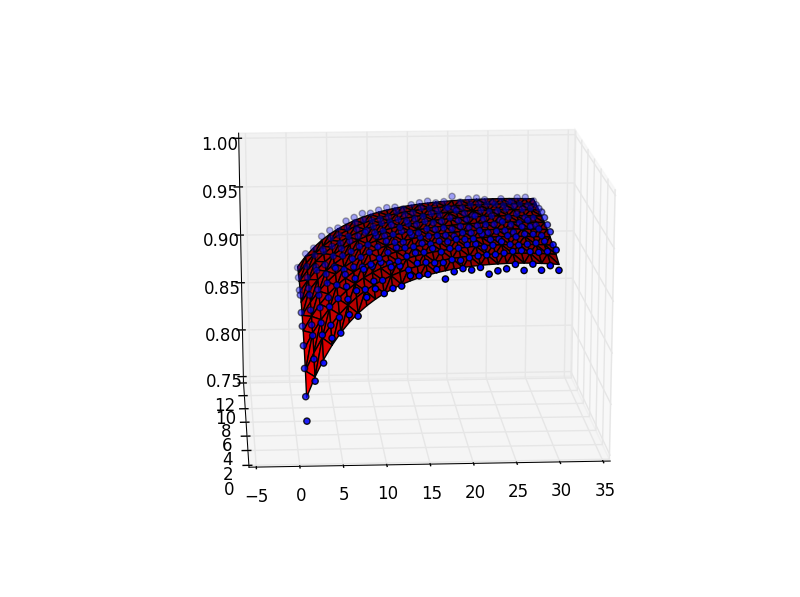
\includegraphics[width=\columnwidth]{../Images/example_result.png}}
\caption{Example Result from Structured.}
\label{icml-historical}
\end{center}
\vskip -0.2in
\end{figure} 


\section{Analysis}
Fully Connected Networks do not add as much accuracy, over parameterized, with quick wins coming with very little connections, and additional ones, adding very little. Something like that.

\section{Future Work}
\begin{itemize}
\item Implementing in different Neural Nets (Convolutional neural nets, are in a sense sparse)
\item Training analysis (does it take longer, shorter, more or less local minima?)
\item Datasets where it succeeds, where it fails
\item More information on topologies vs. sparsity
\item Computational resources were a big limitation
\item Maybe sparsifying intentionally during training (Drop out and Stay out)
\end{itemize}

\section{Conclusion}
Bring home major point : most of NN accuracy, comes with few connections\\
Link to IoT if possible (it's 'hot')



\bibliography{sparse_nn_v1}
\bibliographystyle{icml2015stylefiles/icml2015}

\end{document} 
